\documentclass[a4paper,12pt]{article}
%\documentclass[letterpaper,11pt]{article}
 \setlength{\parskip}{0pc}
 \setlength{\textwidth}{38pc}
 \setlength{\textheight}{56pc} 
 \setlength{\topmargin}{-1.2cm}
 \setlength\oddsidemargin{0cm}  
 \setlength\evensidemargin{0cm} 

\usepackage{setspace}

\usepackage{latexsym} % yw acrescentou

\usepackage[utf8]{inputenc}
\usepackage[english]{babel}

\usepackage{amsfonts,amsmath,amssymb,amsbsy,amsthm,enumerate}
%\usepackage{graphics,graphicx,subfigure,psfrag}

\usepackage[mathscr]{euscript}
%\usepackage{bbm}
%\usepackage{authblk}
%\usepackage{arydshln}
\usepackage{pstricks}
\usepackage{multirow}
\usepackage{verbatim}
\usepackage{color}

\sloppy

\newtheorem{theorem}{Theorem}[section]
\newtheorem{lemma}{Lemma}[section]


\bibliographystyle{plain}

%%TIKZ
\usepackage{tikz}
\usepackage[subrefformat=parens,labelformat=parens]{subcaption}
\usetikzlibrary{calc,positioning,decorations.pathmorphing,decorations.pathreplacing}
\tikzset{black vertex/.style={circle,draw,minimum size=1mm,inner sep=0pt,outer sep=2pt,fill=black, color=black}}
%\tikzset{largepath/.style={orange!75!white,line width=6pt,line cap=round,opacity=0.5}}

%\usepackage{graphicx}

\title{Immersions of cliques in graphs \\ with bounded maximum degree}

\begin{document}

\maketitle

\section{Andrasfai graphs and its relatives}

Andrasfai graphs are well-known triangle-free graphs. 
Any blow-up of an Andrasfai graph is also triangle-free.
So the complement of these graphs have independence number at most 2. 
In what follows we study immersions of cliques in this class of graphs. 
 
Let \(k\) be a positive integer, and let \(F_k\) be the Andrasfai graph of order $k$.
Note that \(h = v(F_k) = 3k-1\) and \(\omega(F_k) = k\).
Let \(G\) be a graph such that \(\overline{G}\) is a blow-up of \(F_k\), 
and let \(V_1,\ldots, V_h\) be the blow-up vertex classes.
Say \(G\) has \(n\) vertices.
Let \(K\) be a maximum clique in \(G\).
One can prove that \(V(K)\) is the disjoint union of precisely \(k\) of the blow-up vertex classes.
Moreover we may assume without loss of generality that \(V(K) = \cup_{i=0}^{k-1} V_{3i+1}\).
In what follows, we find an immersion in \(G\) of a clique in which the branch vertices are 
precisely \(V(G)\setminus V(K)\).

Let \(I = \{2,3,5,6,\ldots,3k-4,3k-3\}\) be the indices of the blow-up vertex classes
corresponding to \(V(G)\setminus V(K)\).
We say a family \(\{A_i: i \in I\}\) of subsets of \(V(K)\) is a \emph{helpful set family} 
if it satisfies the following conditions for every \(i \in I\):
\begin{enumerate}
\item \(|A_i| = |V_i|\);
\item \(A_i \subseteq \overline{N_G(V_i)} \cap V(K)\);
\item the sets \(A_j\) with \(j \in N_{F_k}[i]\cap I\) are mutually disjoint, 
  that is, if \(j,j' \in N_{F_k}[i] \cap I\), then \(A_j\cap A_{j'} = \emptyset\).
\end{enumerate}

\begin{lemma}
  If \(G\) has a helpful set family, then there is an immersion in \(G\) of 
  a clique in which the branch vertices are precisely \(V(G)\setminus V(K)\).
\end{lemma}

\begin{lemma}
  Graph \(G\) has a helpful set family. 
\end{lemma}

This implies the following: 

\begin{theorem}
 The vertex set of the complement of any blow up of an Andrasfai graph can be partitioned 
 into a clique and the branch vertices of an immersion of a clique. 
\end{theorem}


\section{Graphs whose complements admit a special \(3\)-coloring}

\newcommand{\Gcompl}{\overline{G}}

Given a positive integer \(k\),
a \emph{\(k\)-clique-coloring} of a graph \(G\) is a partition \(\{C_1,\ldots, C_k\}\) of \(V(G)\)
such that \(C_i\) is a clique of \(G\) for every \(i\in[k]\).

\begin{theorem}
	Let \(G\) be a graph with \(\alpha(G) = 2\)
	and that admits a \(3\)-clique coloring \(\{C_1,C_2,C_3\}\) such that
	(i) \(C_1\) is a maximum clique of \(G\); and
	(ii) \(G[C_2\cup C_3]\) has no induced \(C_4\).
	Then \(G\) contains an immersion of a clique whose set of branch vertices is precisely \(C_2\cup C_3\).
\end{theorem}

\begin{proof}
	Observe that \(C_1,C_2,C_3\) is a \(3\)-coloring of \(\Gcompl\),
	and by hypothesis \(C_1\) is a maximum independent set of \(\Gcompl\).
	Let \(i\in\{2,3\}\) and let \(C\subseteq C_i\).
	If \(|N_{C_1}(C)| < |C|\), 
	then \((C_1\setminus N_{C_1}(C))\cup C\) is an independent set that is larger than \(C_1\),
	a contradiction to the maximality of \(C_1\).
	Then \(|N_{C_1}(C)| \geq |C|\) for any subset of \(C_i\).
	By Hall's Theorem, there is a matching \(M_i\) in \(\Gcompl[C_i,C_1]\) that covers \(C_i\).
	
	Given a vertex \(u\in C_2 \cup C_3\), 
	note that there is precisely one edge in \(M_2\cup M_3\) that contains \(u\),
	and let \(r_u\in C_1\) be the vertex such that \(ur_u\in M_2\cup M_3\).
%	We say that \(r_u\) is the \emph{representative} of \(u\).
	Note that \(r_u \notin N(u)\),
	and hence, since \(\alpha(G) = 2\), \(r_u\) is adjacent to every vertex in \(V(G)\setminus N[u]\).
	In what follows, let \(E' = E\big(G[C_2,C_3]\big)\).
	Note that if \(u\in C_2\) and \(v\in C_3\) are such that \(r_u = r_v = w\),
	then \(uv \in E'\), otherwise \(u,v,w\) would be an independent set of size \(3\).
%	
	Note that if \(uv\notin E'\) we have \(r_u\in N(v)\), \(r_v\in N(u)\),
	and since \(C_1\) is a clique, \(r_ur_v\in E(G)\).

	Now, for every \(uv\notin E'\), let \(P_{uv}\) be the path \(u r_v r_u v\).
	We claim that the paths \(P_e\) with \(e\notin E'\) are pairwise edge-disjoint.
	Indeed, let \(u,u' \in C_2\) and \(v,v' \in C_3\) be such that \(uv,u'v' \notin E'\)
	and \(uv \neq u'v'\).
	Note that \(u\) and \(u'\) (resp. \(v\) and \(v'\)) are not necessarily distinct,
	but either \(u \neq u'\) or \(v \neq v'\).
	If \(v\neq v'\), then \(r_v \neq r_{v'}\) because \(M_3\) is a matching.
	This implies that \(ur_v \neq u'r_{v'}\) (even if \(u = u'\)).
	Analogously, we have \(vr_u \neq v'r_{u'}\).
	In what follows, we prove that \(r_ur_v \neq r_{u'}r_{v'}\).
	Suppose, for a contradiction, that \(r_ur_v = r_{u'}r_{v'}\).
	If \(r_u = r_{u'}\) and \(r_v = r_{v'}\), then \(u=u'\) and \(v=v'\), a contradiction.
	Thus, we may assume \(r_u = r_{v'}\) and \(r_v = r_{u'}\).
	As noted above, this implies that \(uv',vu' \in E'\) (see Figure~\ref{fig:induced-C4}).
	But then \(\{u,v,u',v'\}\) induce a \(C_4\) in \(G[C_2\cup C_3]\),
	a contradiction .
\end{proof}

\begin{figure}[ht]
    \centering
        \centering
        \begin{tikzpicture}[scale = 0.8]
        
        \node (u)	[black vertex] at	(-2,-1)	{};
        \node (u')	[black vertex] at	(-2,1)	{};
        \node (v)	[black vertex] at	(2,-1)	{};
        \node (v')	[black vertex] at	(2,1)	{};
        \node (ru)	[black vertex] at	(1,3)	{};
        \node (rv)	[black vertex] at	(-1,3)	{};
        
        \node [anchor=north]		at		(u)		{$u$};
        \node [anchor=south east]	at		(u')	{$u'$};
        \node [anchor=north]		at		(v)		{$v$};
        \node [anchor=south west]	at		(v')	{$v'$};
        \node [anchor=north]		at		(ru)	{$r_u$};
        \node [anchor=north]		at		(rv)	{$r_v$};
        \node [anchor=south east]	at		(ru)	{$r_{v'}$};
        \node [anchor=south west]	at		(rv)	{$r_{u'}$};

        
        \draw [thick] (u) -- (u') (v) -- (v') (ru) -- (rv);
        \draw [thick] (ru) to [bend left = 90] (v) (ru) -- (u');
        \draw [thick] (rv) to [bend right = 90] (u) (rv) -- (v');
        \draw [thick,dashed] (u) -- (v) (u') -- (v');
        \draw [thick] (u) -- (v') (v) -- (u');
        \draw [thick,dashed] (u) to [bend left = 15] (ru) (v) to [bend right = 15] (rv) (u') to [bend left] (rv) (v') to [bend right] (ru);
        \end{tikzpicture}
    \caption{}
    \label{fig:induced-C4}
\end{figure}
%\bibliographystyle{amsplain}

%\bibliography{bibliografia}

\end{document}
